\documentclass[aspectratio=169,fleqn]{beamer}
\usepackage{spc}
\usepackage{graphicx}
\newcommand\cran[1]{\blue\href{https://cran.r-project.org/web/#1}}
\begin{document}

\begin{frame}
  \title{\vspace{-5ex}\darkblue Scoping the next stock assessment
    platform\\[2ex]
    \it\large\darkgray
    Project 123 progress update and outline of options}
  \author{\vspace{-10ex}\darkgray\bf
    Arni Magnusson, Nick Davies,\\[0.5ex]
    Graham Pilling, Paul Hamer}
  \date{\darkgreen SPC Pre-Assessment Workshop (PAW)\\[0.5ex]
    Nouméa, 10 April 2025}
  \titlepage
\end{frame}

% ______________________________________________________________________________

\begin{frame}{Overview}
  \begin{itemize}
    \item[] {\bf\darkblue Overall Plan} \comment{migrating from MFCL, project
      outline, objectives,\\
      \h{17.1ex}activities, timeline}\\[5ex]
    \item[] {\bf\darkblue SC20 in 2024} \comment{international expert meeting,
      overview of software}\\[5ex]
    \item[] {\bf\darkblue Latest Developments} \comment{workshop in Aug 2024,
      multiple-criteria decision analysis,\\
      \h{27ex}external analysis of tagging data, workshop in May 2025}\\[5ex]
    \item[] {\bf\darkblue SC21 in 2025} \comment{evaluation of model features,
      outline of options,\\
      \h{18.5ex}required resources}\\[1ex]
  \end{itemize}
\end{frame}

% ______________________________________________________________________________

\begin{frame}{The need to to migrate to new software}
  \begin{itemize}
    \item[] MULTIFAN-CL (MFCL) has been used in SPC tuna assessments since
    1990s\\[4ex]
    \item[] MFCL team (Dave Fournier, John Hampton, Nick Davies) retiring in the
    2020s\\[4ex]
    \item[] Development of new features is slowing down\\[4ex]
    \item[] Resources are being allocated to succession plans\\[2ex]
  \end{itemize}
\end{frame}

% ______________________________________________________________________________

\begin{frame}{Migrating all MFCL assessments to other platforms}
  \textbf{\darkgreen Shared} process, {\darkgreen\bf continuous} communications,
  {\darkgreen\bf adaptive} strategy\\[2ex]
  \begin{itemize}
    \item[] {\blue\bf WCPFC} ~--~ guidance\\[2ex]
    \item[] {\blue\bf SPC} ~--~ conduct and coordinate the work\\[3ex]
  \end{itemize}
  Also involved: other tuna RFMOs and various research labs\\[4ex]
  Swordfish and striped marlin assessments migrating to Stock Synthesis in
  2025\\[4ex]
  Tuna assessments in MFCL, currently evaluating alternative platforms and\\
  development options\\[1ex]
\end{frame}

% ______________________________________________________________________________

\begin{frame}{Project outline}
  This scoping project is scheduled from 1 Feb 2024 to 31 Dec 2026. It
  will:\\[3ex]
  \begin{itemize}
    \item[] Evaluate features and capabilities that will be important in future
    tuna assessments\\[3ex]
    \item[] Explore fitting models to tuna data using existing software
    platforms\\[3ex]
    \item[] Guide decisions on what kind of new software development will be
    required\\[3ex]
    \item[] Establish collaboration with tuna RFMOs and research labs to achieve
    these goals\\[3ex]
  \end{itemize}
\end{frame}

% ______________________________________________________________________________

\begin{frame}{Objectives}
  The ideal outcome would be that in 10--15 years, the WCPFC tuna assessments\\
  are conducted in software that has the following three characteristics or
  criteria:\\[1ex]
  \begin{enumerate}
    \item {\bf\blue Scientific quality}: has good estimation performance, makes
    good use\\
    of available data, allows spatial and temporal variability in processes,\\
    runs fast.\\[1.5ex]
    \item {\bf\blue Beginner friendly}: new staff scientists can conduct a stock
    assessment\\
    in their first year of contract, configuring and understanding the
    models.\\[1.5ex]
    \item {\bf\blue Widely used}: large development team and user community
    beyond SPC,\\
    new staff scientists can find expert help outside of SPC, tools
    to work\\
    with model input and output are feature complete and maintained
    outside\\
    of SPC, external reviewers have a good understanding of model\\
    configurations and options.\\[2ex]
  \end{enumerate}
\end{frame}

% ______________________________________________________________________________

\begin{frame}{Scoping project and possible follow-up projects}
  \vspace{-1ex}
  ~\h{-3ex}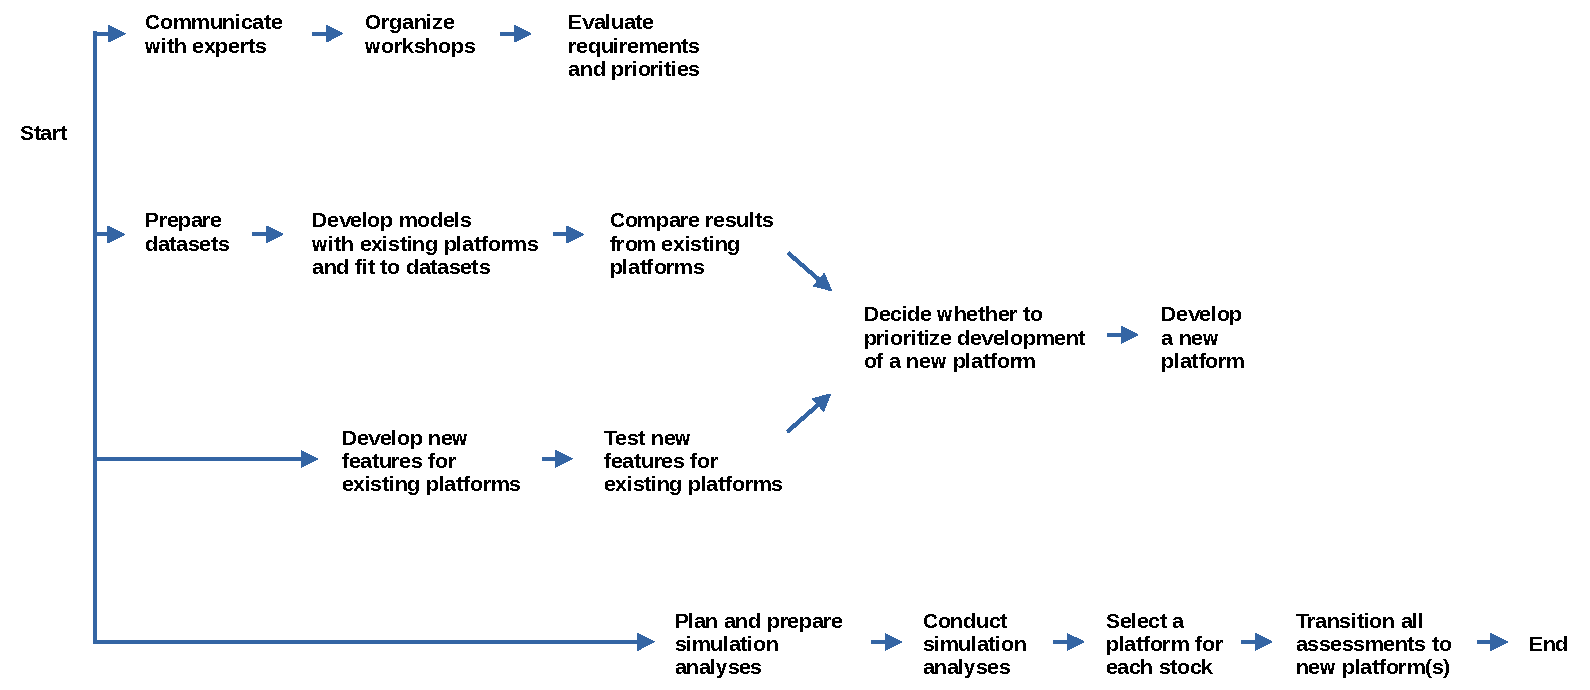
\includegraphics[width=1.05\textwidth]{p123_diagram}
\end{frame}

% ______________________________________________________________________________

\begin{frame}{2024 project activities}
  \begin{itemize}
    \item[] Scoping project launched (Feb)\\[3ex]
    \item[] PAW discussion (Mar)\\[3ex]
    \item[] International expert meeting (May--Jun)\\[3ex]
    \item[] SC20 discussion (Aug)\\[3ex]
    \item[] Developer workshop (Aug)\\[3ex]
    \item[] Follow up with tuna RFMOs and research labs (Dec)\\[2ex]
  \end{itemize}
\end{frame}

% ______________________________________________________________________________

\begin{frame}{2025 project activities}
  \begin{itemize}
    \item[] Evaluation of RTMB as a development platform (Jan--Feb)\\[3ex]
    \item[] PAW discussion (Apr)\\[3ex]
    \item[] Follow up with tuna RFMOs and research labs (Apr)\\[3ex]
    \item[] Spatio-temporal tagging model workshop (May)\\[3ex]
    \item[] SC21 discussion (Aug)\\[3ex]
    \item[] Model development workshop (Quarter 4)\\[2ex]
  \end{itemize}
\end{frame}

% ______________________________________________________________________________

\begin{frame}{2026 draft plan}
  \begin{itemize}
    \item[] Evaluation of external analysis of tagging data (Quarter 1)\\[2ex]
    \item[] PAW discussion (Apr)\\[2ex]
    \item[] Model development workshop (Quarter 2)\\[2ex]
    \item[] Follow up with tuna RFMOs and research labs (Quarter 2)\\[2ex]
    \item[] SC22 discussion, final report of P123 (Aug)\\[2ex]
    \item[] $\Rightarrow$ Launch a project similar to P123, {\green
      coordinating} activities related to\\
    \phantom{$\Rightarrow$} the migration of assessments and related research \&
    development\\[2ex]
    \item[] $\Rightarrow$ Launch collaborative projects {\green conducting} work
    related to the\\
    \phantom{$\Rightarrow$} development of next-generation assessment
    models\\[2ex]
  \end{itemize}
\end{frame}

% ______________________________________________________________________________

\begin{frame}{Overview}
  \begin{itemize}
    \item[] {\bf\darkblue Overall Plan} \comment{migrating from MFCL, project
      outline, objectives,\\
      \h{17.1ex}activities, timeline}\\[5ex]
    \item[] {\bf\darkblue SC20 in 2024} \comment{international expert meeting,
      overview of software}\\[5ex]
    \item[] {\bf\darkblue Latest Developments} \comment{workshop in Aug 2024,
      multiple-criteria decision analysis,\\
      \h{27ex}external analysis of tagging data, workshop in May 2025}\\[5ex]
    \item[] {\bf\darkblue SC21 in 2025} \comment{evaluation of model features,
      outline of options,\\
      \h{18.5ex}required resources}\\[1ex]
  \end{itemize}
\end{frame}

% ______________________________________________________________________________

\begin{frame}{Recommendations from 2024 international expert meeting}
  \begin{enumerate}
    \item {\darkgreen\bf Tuna} assessment software\\
    \comment{\gray design and develop a model specific for tuna
      assessments}\\[1ex]
    \item {\darkgreen\bf RTMB} programming environment\\
    \comment{\gray lean software development paradigm, maybe a specific model
      for each species}\\[1ex]
    \item {\darkgreen\bf State-space} formulation\\
    \comment{\gray statistically and computationally efficient way to allow
      time-varying processes}\\[1ex]
    \item {\darkgreen\bf Age-length} structure\\
    \comment{\gray explicitly track the population by age and length, if not too
      costly}\\[1ex]
    \item {\darkgreen\bf Simple} models\\
    \comment{\gray short-term staff, young scientists, simple user interface,
      simpler models}\\[1ex]
    \item {\darkgreen\bf Collaboration} between tuna RFMOs\\
    \comment{\gray MFCL and Stock Synthesis in a sunset phase, data analyses
      comparable between RFMOs}\\[1.5ex]
  \end{enumerate}
\end{frame}

% ______________________________________________________________________________

\begin{frame}{Stock assessment software}
  Existing software, ready for multi-region tuna assessments\\[3ex]
  \begin{itemize}
    \item[-] {\darkgreen\bf Stock Synthesis} is used by IATTC, IOTC, and
    ICCAT\\[3ex]
    \item[-] {\darkgreen\bf Gadget} has many features relevant for tuna
    assessments\\[3ex]
    \item[-] {\darkgreen\bf Casal} has many features relevant for tuna
    assessments\\[4ex]
  \end{itemize}
  These could be extended further as needs arise\\[2ex]
\end{frame}

% ______________________________________________________________________________

\begin{frame}{Stock assessment software}
  Software that could be developed further:\\[3ex]
  \begin{itemize}
    \item[-] {\darkgreen\bf sbt} is built around CKMR, currently for
    single-region assessments\\[3ex]
    \item[-] {\darkgreen\bf ALSCL} is a state-space model that fits length
    comps, currently no catches\\[3ex]
    \item[-] {\darkgreen\bf WHAM$\,$\raisebox{0.15ex}{+}$\,$Length} is a
    state-space that fits length comps, currently single-region\\[3ex]
    \item[-] {\darkgreen\bf SAM$\,$\raisebox{0.15ex}{+}$\,$Length} is an early
    exploration of extending SAM to fit length comps\\[3ex]
    \item[-] {\darkgreen\bf Stock Synthesis$\,$\raisebox{0.15ex}{+}$\,$Enhanced
      Tags} is a proposed enhancement of the tag module\\[2ex]
  \end{itemize}
\end{frame}

% ______________________________________________________________________________

\begin{frame}{Stock assessment software}
  Also relevant:\\[4ex]
  \begin{itemize}
    \item[-] {\darkgreen\bf Stock Synthesis$\,$\raisebox{0.15ex}{+}$\,$CKMR} is
    an experimental add-on, not included in core software\\[4ex]
    \item[-] {\darkgreen\bf FIMS}, NOAA project coordinating the development of
    a next-generation framework\\[6ex]
  \end{itemize}
\end{frame}

% ______________________________________________________________________________

\begin{frame}{Stock Synthesis}
  \textit{\blue Cons}
  \begin{itemize}
    \item[--] fewer features than MFCL\\[1ex]
    \item[--] old software, but will be used in tuna assessments until a
    next-generation\\
    software platform comes about\\[1.5ex]
  \end{itemize}
  \textit{\blue Pros}
  \begin{itemize}
    \item[+] used by IATTC, IOTC, ICCAT, and ISC (and NOAA, ICES, GFCM,
    CSIRO, etc.)\\[1ex]
    \item[+] facilitates collaboration between the tuna RFMOs, including future
    development\\[1ex]
    \item[+] shortens training time for new SPC staff, makes skills and
    experience transferable\\[1ex]
    \item[+] large user community, relevant for peer reviews and discussing
    technical decisions\\[1ex]
    \item[+] exceptionally complete suite of tools, diagnostics, automated plots
    and tables\\[1ex]
    \item[+] next-generation frameworks will support transitioning from Stock
    Synthesis\\[1ex]
  \end{itemize}
\end{frame}

% ______________________________________________________________________________

\begin{frame}{Overview}
  \begin{itemize}
    \item[] {\bf\darkblue Overall Plan} \comment{migrating from MFCL, project
      outline, objectives,\\
      \h{17.1ex}activities, timeline}\\[5ex]
    \item[] {\bf\darkblue SC20 in 2024} \comment{international expert meeting,
      overview of software}\\[5ex]
    \item[] {\bf\darkblue Latest Developments} \comment{workshop in Aug 2024,
      multiple-criteria decision analysis,\\
      \h{27ex}external analysis of tagging data, workshop in May 2025}\\[5ex]
    \item[] {\bf\darkblue SC21 in 2025} \comment{evaluation of model features,
      outline of options,\\
      \h{18.5ex}required resources}\\[1ex]
  \end{itemize}
\end{frame}

% ______________________________________________________________________________

\begin{frame}{Scoping project workshop (Aug 2024)}
  Matapouri, 26-30 August 2024\\[1ex]
  Arni Magnusson, Nick Davies\\[3ex]
  \textbf{Objectives}\\[1.5ex]
  \begin{itemize}
    \item[] {\green Project discussion}: objectives, options, possible outcomes,
    and other\\
    \h{18.1ex}project-level topics\\[2ex]
    \item[] {\green Simulation study}: discuss objectives and study design,
    related to\\
    \h{17.2ex}future software development\\[2ex]
    \item[] {\green Technical explorations}: TMB automatic sparseness
    detection,\\
    \h{22.1ex}RTMB fisheries examples and modular design,\\
    \h{22.1ex}and tagging model in MFCL\\[2.5ex]
  \end{itemize}
\end{frame}

% ______________________________________________________________________________

\begin{frame}{Scoping project workshop (Aug 2024)}
  Matapouri, 26-30 August 2024\\[1ex]
  Arni Magnusson, Nick Davies\\[3ex]
  \h{1.2ex}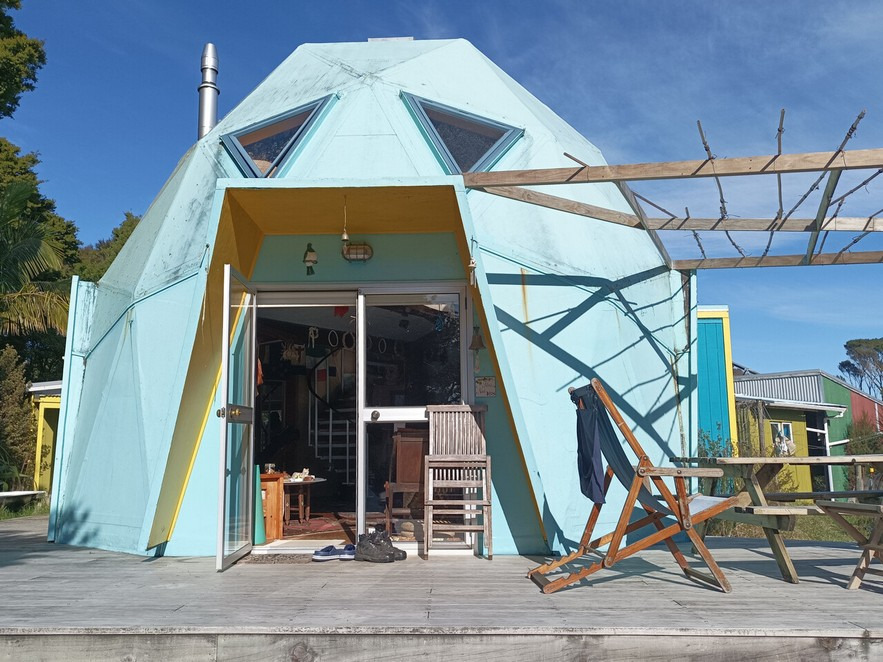
\includegraphics[width=0.45\textwidth]{matapouri_house}\qquad
  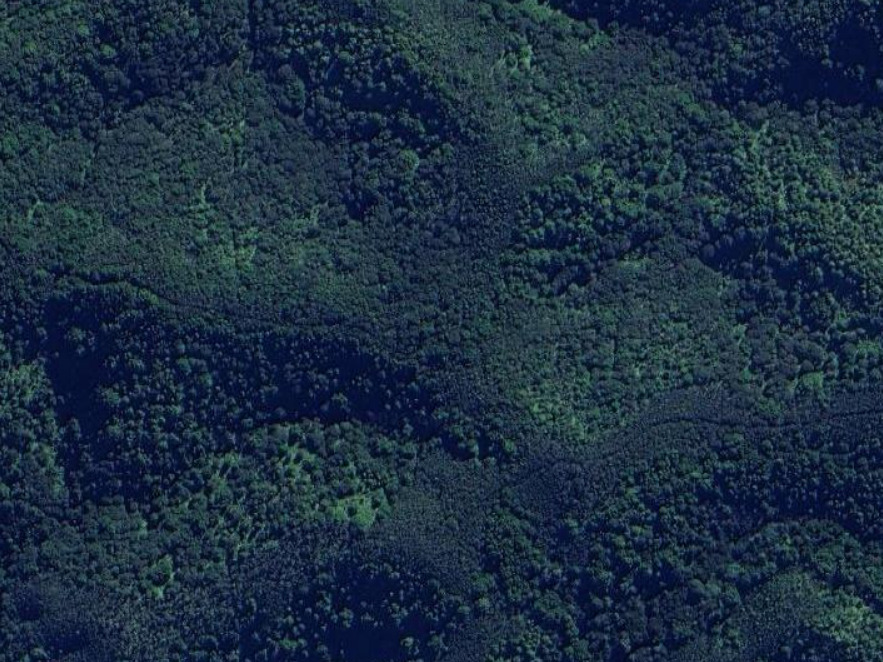
\includegraphics[width=0.45\textwidth]{matapouri_map}
  \vspace{2.6ex}
\end{frame}

% ______________________________________________________________________________

\begin{frame}{Objectives}
  The ideal outcome would be that in 10--15 years, the WCPFC tuna assessments\\
  are conducted in software that has the following three characteristics or
  criteria:\\[1ex]
  \begin{enumerate}
    \item {\bf\blue Scientific quality}: has good estimation performance, makes
    good use\\
    of available data, allows spatial and temporal variability in processes,\\
    runs fast.\\[1.5ex]
    \item {\bf\blue Beginner friendly}: new staff scientists can conduct a stock
    assessment\\
    in their first year of contract, configuring and understanding the
    models.\\[1.5ex]
    \item {\bf\blue Widely used}: large development team and user community
    beyond SPC,\\
    new staff scientists can find expert help outside of SPC, tools
    to work\\
    with model input and output are feature complete and maintained
    outside\\
    of SPC, external reviewers have a good understanding of model\\
    configurations and options.\\[2ex]
  \end{enumerate}
\end{frame}

% ______________________________________________________________________________

\begin{frame}{Multiple-criteria decision analysis}
  The three criteria incur conflict in their achievement, and inevitable
  trade-offs\\
  are required when considering the various options for future
  platforms. Consider\\
  the following three existing platforms:\\[2ex]
  \begin{tabular}{ll}
    \blue MFCL      & The main problems in the near future are related to the
                      criteria 2 and 3.\\
    ~               & The current usage of MFCL already meets criterion
                      1.\\[2ex]
    \blue Gadget    & Gadget could perhaps provide an incremental improvement in
                      criterion 1\\
    ~               & but would perhaps not solve the problems in meeting
                      criteria 2 and 3.\\[2ex]
    \blue Stock     & Migrating tuna assessments from MFCL to Stock Synthesis
                      could be a\\
    \blue Synthesis & partial sacrifice in criterion 1 to greatly improve
                      criteria 2 and 3.\\[3ex]
  \end{tabular}
  Noting that the comments in respect of the above three scenarios are subject
  to further explorations and a simulation study.\\[2ex]
\end{frame}

% ______________________________________________________________________________

\begin{frame}{Long-term possible outcomes}
  In 10--15 years, the WCPFC tuna assessments could be conducted in:\\[1ex]
  \begin{itemize}
    \item[-] {\blue Stock Synthesis}
    \item[-] {\blue Gadget}
    \item[-] New software developed independently by {\blue SPC}
    \item[-] New software developed jointly by {\blue tuna RFMOs}, independent
    of FIMS
    \item[-] New software developed jointly by tuna RFMOs, linked with
    {\blue FIMS} libraries
    \item[-] {\blue Other} new software that may come about\\[2ex]
  \end{itemize}

  Other tuna stock assessments around the world (IATTC, IOTC, ICCAT, ISC)\\
  use Stock Synthesis and will probably continue to do so until a
  next-generation framework comes about, which could be FIMS\\[2ex]
\end{frame}

% ______________________________________________________________________________

\begin{frame}{Evaluation of RTMB as a model development platform}
  \textbf{\blue Scripts}\\[0.5ex]
  \begin{itemize}
    \item[] {\green RTMB} is a recent R package, providing a streamlined
    interface for TMB\\[1.5ex]
    \item[] The skipjack growth project was using TMB scripts and used the
    opportunity\\
    to convert the analysis to RTMB scripts, in order to compare RTMB and
    TMB\\[1.5ex]
    This resulted in {\green streamlined code} that runs equally fast and gives
    the same result\\
    as the original TMB scripts\\[1.5ex]
    No compilation required, considerably easier to develop and modify
    models\\[1.5ex]
    $\Rightarrow$ RTMB can be {\green recommended} as a better alternative to
    TMB for most scripts\\[3ex]
  \end{itemize}
  \textbf{\blue Package}\\[0.5ex]
  \begin{itemize}
    \item[] The next step was to evaluate RTMB as the basis of a {\green model
      package}\\[3ex]
  \end{itemize}
\end{frame}

% ______________________________________________________________________________

\begin{frame}{fishgrowth: Fit Growth Curves to Fish Data}
  \rm\scriptsize\fontfamily{ptm}\selectfont Fit growth models to otoliths and/or
  tagging data, using the 'RTMB' package and maximum likelihood. The\\
  otoliths (or similar measurements of age) provide direct observed coordinates
  of age and length. The tagging\\
  data provide information about the observed length at release and length at
  recapture at a later time, where\\
  the age at release is unknown and estimated as a vector of parameters. The
  growth models provided by this\\
  package can be fitted to otoliths only, tagging data only, or a combination of
  the two. Growth variability can\\
  be modelled as constant or increasing with length.\\[1.2ex]
  \begin{tabular}{ll}
    Version: & 1.0.2\\[0.1ex]
    Depends: & R ($\geq$ 2.10), \cran{packages/RTMB/index.html}{RTMB}\\[0.1ex]
    Suggests: & \cran{packages/areaplot/index.html}{areaplot}\\[0.1ex]
    Published: & 2024-04-08\\[0.1ex]
    DOI: & \blue\href{https://doi.org/10.32614/CRAN.package.fishgrowth}%
           {10.32614/CRAN.package.fishgrowth}\\[0.1ex]
    Author: & Arni Magnusson [aut, cre], Mark Maunder [aut]\\[0.1ex]
    Maintainer: & Arni Magnusson $<$thisisarni at gmail.com$>$\\[0.1ex]
    License: & \cran{licenses/GPL-3}{GPL-3}\\[0.1ex]
    URL: & \green\href{https://github.com/arni-magnusson/fishgrowth}%
           {https://github.com/arni-magnusson/fishgrowth}\\[0.1ex]
    NeedsCompilation: & no\\[0.1ex]
    Materials: & \cran{packages/fishgrowth/news/news.html}{NEWS}\\[0.1ex]
    CRAN checks: & \cran{checks/check_results_fishgrowth.html}%
                   {fishgrowth results}\\[0.1ex]
  \end{tabular}
  ~\\[0.5ex]
  Documentation:\\[1ex]
  \begin{tabular}{ll}
    Reference manual:
    & \cran{packages/fishgrowth/fishgrowth.pdf}{fishgrowth.pdf}\\[2ex]
  \end{tabular}
\end{frame}

% ______________________________________________________________________________

\begin{frame}{External analysis of tagging data}
  \begin{itemize}
    \item[] P123 reaching out in December 2024 to Mark Maunder (IATTC) who
    provided:\\[0.5ex]
    \begin{enumerate}\normalsize
      \item Useful comments on the initial ideas of a simulation study
      design\\[1ex]
      \item Recommendation that SPC consider the possibility that post-MFCL
      assessments might analyze tags outside the stock assessment model\\[3ex]
    \end{enumerate}
    \item[] IATTC has recently employed a new Mildenberger-Nielsen (2022, 2023,
    2024)\\[0.2ex]
    spatio-temporal model to analyze skipjack tags in the Eastern Pacific
    Ocean\\[3ex]
    \item[] Incorporated in the IATTC EPO skipjack 2024 assessment\\[4ex]
    $\Rightarrow$ Spatio-temporal model produces a {\green biomass index},
    overall or by region,\\[0.2ex]
    \phantom{$\Rightarrow$} that can be incorporated into {\green any stock
      assessment platform}\\[3ex]
  \end{itemize}
\end{frame}

% ______________________________________________________________________________

\begin{frame}{External analysis of tagging data}
  \centering
  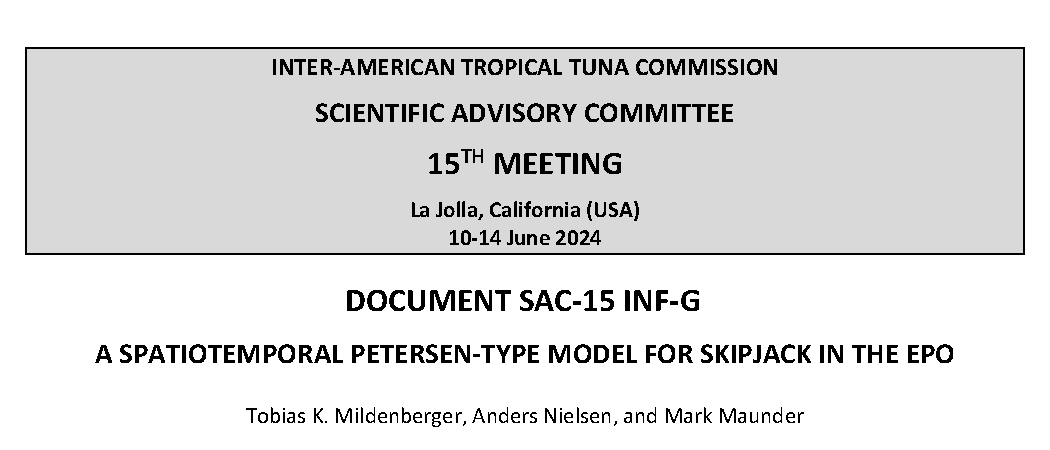
\includegraphics[width=0.85\textwidth]{iattc_report}
\end{frame}

% ______________________________________________________________________________

\begin{frame}{External analysis of tagging data}
  \textbf{\darkgreen SPC-DTU Workshop 2025}\\[2ex]
  Copenhagen, 12--16 May 2025\\[2ex]
  Anders Nielsen, Arni Magnusson, Inna Senina,\\[0.2ex]
  Joe Scutt Phillips, Tobias Mildenberger\\[3ex]
  \textbf{Objective}\\[1ex]
  \begin{itemize}
    \item[] Explore the possibility of applying the Mildenberger-Nielsen
    spatio-temporal\\
    tagging model to SPC tagging data. The end product of such an analysis\\
    could be a region-specific abundance index that can be incorporated in a\\
    tuna stock assessment. The workshop will focus on skipjack tuna in the\\
    western and central Pacific Ocean.\\[2ex]
  \end{itemize}
\end{frame}

% ______________________________________________________________________________

\begin{frame}{Overview}
  \begin{itemize}
    \item[] {\bf\darkblue Overall Plan} \comment{migrating from MFCL, project
      outline, objectives,\\
      \h{17.1ex}activities, timeline}\\[5ex]
    \item[] {\bf\darkblue SC20 in 2024} \comment{international expert meeting,
      overview of software}\\[5ex]
    \item[] {\bf\darkblue Latest Developments} \comment{workshop in Aug 2024,
      multiple-criteria decision analysis,\\
      \h{27ex}external analysis of tagging data, workshop in May 2025}\\[5ex]
    \item[] {\bf\darkblue SC21 in 2025} \comment{evaluation of model features,
      outline of options,\\
      \h{18.5ex}required resources}\\[1ex]
  \end{itemize}
\end{frame}

% ______________________________________________________________________________

\begin{frame}{SC21 in 2025}
  Two main options seem particularly relevant at this point\\[2ex]
  \begin{tabular}{llllll}
    \blue ~1. & MFCL & $\rightarrow$ & Stock Synthesis & $\rightarrow$
    & Next-generation\\[2ex]
    \blue ~2. & MFCL & $\rightarrow$ & Wait . . .      & $\rightarrow$
    & Next-generation\\
  \end{tabular}
  ~\\\vspace{3.5ex}
  Between PAW (April) and SC21 (August)\\[1ex]
  \begin{itemize}
    \item[-] Elaborate on the benefits, drawbacks, uncertainties,\\
    and required resources related to the above options\\[1.5ex]
    \item[-] Explore the possibility of analyzing the tagging data\\
    outside of the stock assessment model\\[1.5ex]
    \item[-] Evaluate features and capabilities that will be\\
    important in future tuna assessments\\[1.5ex]
  \end{itemize}
\end{frame}

% ______________________________________________________________________________

\begin{frame}{Project website}
  \centering\small
  \textblue{\url{https://github.com/PacificCommunity/ofp-sam-transition-plan}}
\end{frame}

% ______________________________________________________________________________

\begin{frame}{Summary}
  \begin{itemize}
    \item[] {\bf\darkblue Overall Plan} \comment{migrating from MFCL, project
      outline, objectives,\\
      \h{17.1ex}activities, timeline}\\[5ex]
    \item[] {\bf\darkblue SC20 in 2024} \comment{international expert meeting,
      overview of software}\\[5ex]
    \item[] {\bf\darkblue Latest Developments} \comment{workshop in Aug 2024,
      multiple-criteria decision analysis,\\
      \h{27ex}external analysis of tagging data, workshop in May 2025}\\[5ex]
    \item[] {\bf\darkblue SC21 in 2025} \comment{evaluation of model features,
      outline of options,\\
      \h{18.5ex}required resources}\\[1ex]
  \end{itemize}
\end{frame}

\end{document}
